\href{https://github.com/mfclabber/itmo-cv-labs/tree/main/lab4}{Исходный код на GitHub}. 

Для удобства отладки и сборки используется средство автоматизации сборки ПО CMake:
\begin{lstlisting}[style=cpp_white, caption={CMakeLists.txt для сборки проекта}]
cmake_minimum_required(VERSION 2.8)

project( CV_LW4 )
find_package( OpenCV REQUIRED )

include_directories( ${OpenCV_INCLUDE_DIRS} )
add_executable( ${PROJECT_NAME}  src/lab2.cpp )

target_link_libraries( ${PROJECT_NAME} ${OpenCV_LIBS} )
\end{lstlisting}

\section{Бинаризация}

\subsection{Бинаризация по порогу}

Простейшим способом сегментации изображения на два класса (фоновые пиксели и пиксели объекта) является бинаризация. Би-
наризацию можно выполнить по порогу или по двойному порогу. Впервом случае:

\begin{equation}
    I_{new}(x, y) = \begin{cases}
        0, & I(x, y) \leq t \\[1pt]
        1, &I(x, y) > t,\\[1pt]
    \end{cases} 
\label{eq:complex_func}
\end{equation}
где $I$ — исходное изображение, $I_{new}$ — бинаризованное изображе-
ние, $t$ — порог бинаризации.

\begin{lstlisting}[style=cpp_white, caption={Исходный код для бинаризации}]
cv::threshold(image, image_new, 127, 255, cv::THRESH_BINARY);

cv::imwrite(path + "/outputs/image_binarization.png", image_new);
cv::imshow("image", image_new);
cv::waitKey();
\end{lstlisting}

\pagebreak

\begin{figure}[ht]
    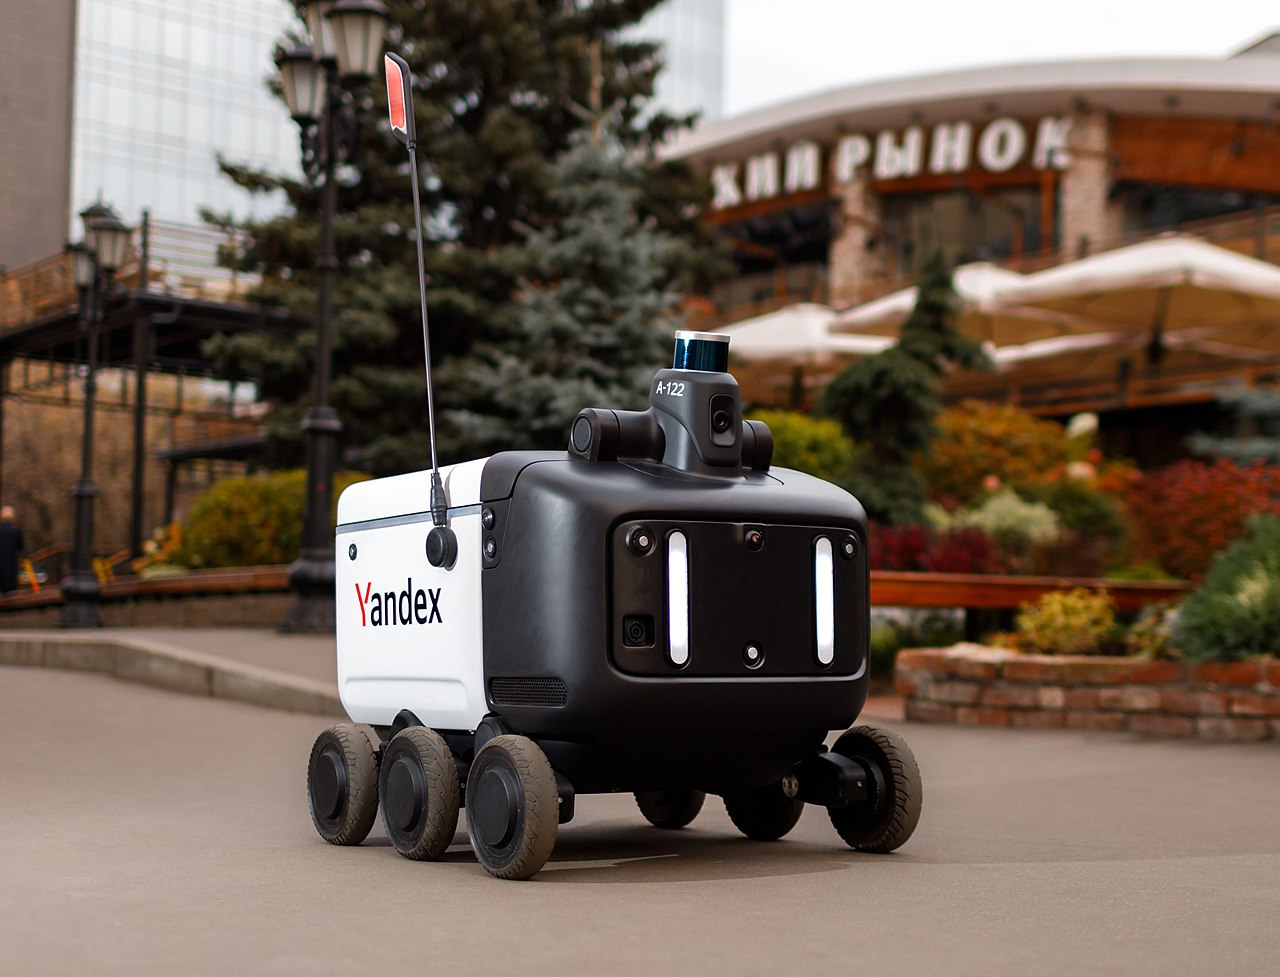
\includegraphics[width=\textwidth]{../source/yandex_delivery_robot.png}
    \caption{Исходное изображение}
    \label{fig:source_image}
\end{figure}

\begin{figure}[ht]
    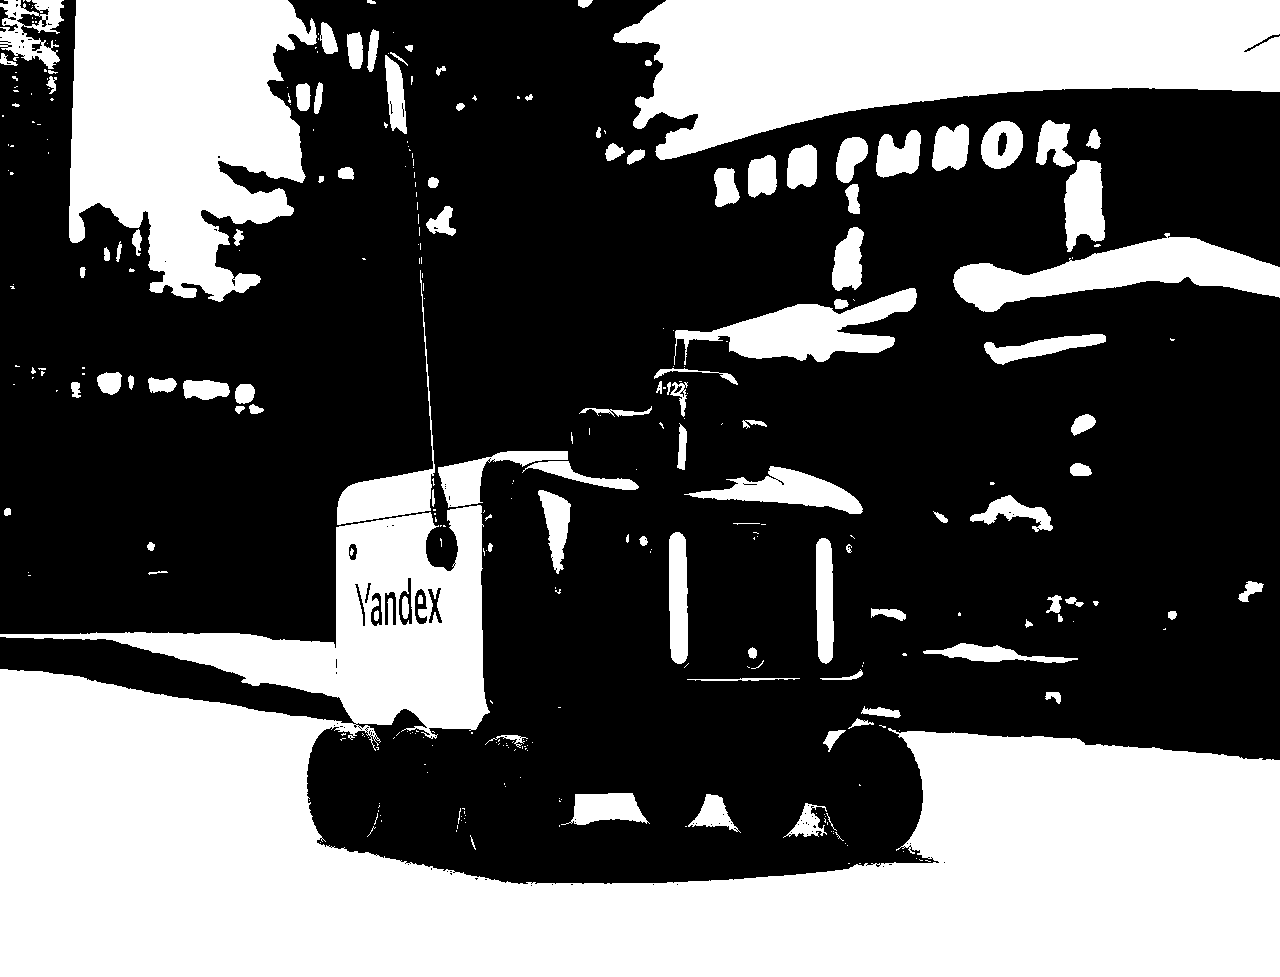
\includegraphics[width=\textwidth]{../outputs/image_binarization.png}
    \caption{Бинаризованное изображение}
    \label{fig:р}
\end{figure}

\pagebreak

\subsection{Бинаризация по двойному порогу}

\begin{equation}
    I_{new}(x, y) = \begin{cases}
        0, & I(x, y) \leq t_1 \\[1pt]
        1, & t_1 < I(x, y) \leq t_2,\\[1pt]
        1, & I(x, y) > t_2,\\[1pt]
    \end{cases} 
\label{eq:complex_func}
\end{equation}

где $I$ — исходное изображение, $I_{new}$ — бинаризованное изображе-
ние, $t1$ и $t2$ — верхний и нижний пороги бинаризации.

\begin{lstlisting}[style=cpp_white, caption={Исходный код для бинаризации по двойному порогу}]
cv::threshold(image, image_new, 127, 255, cv::THRESH_TOZERO);
cv::threshold(image_new, image_new, 200, 255, cv::THRESH_BINARY);

cv::imwrite(path + "/outputs/image_double_binarization.png", image_new);
cv::imshow("image", image_new);
cv::waitKey();
\end{lstlisting}

\begin{figure}[ht]
    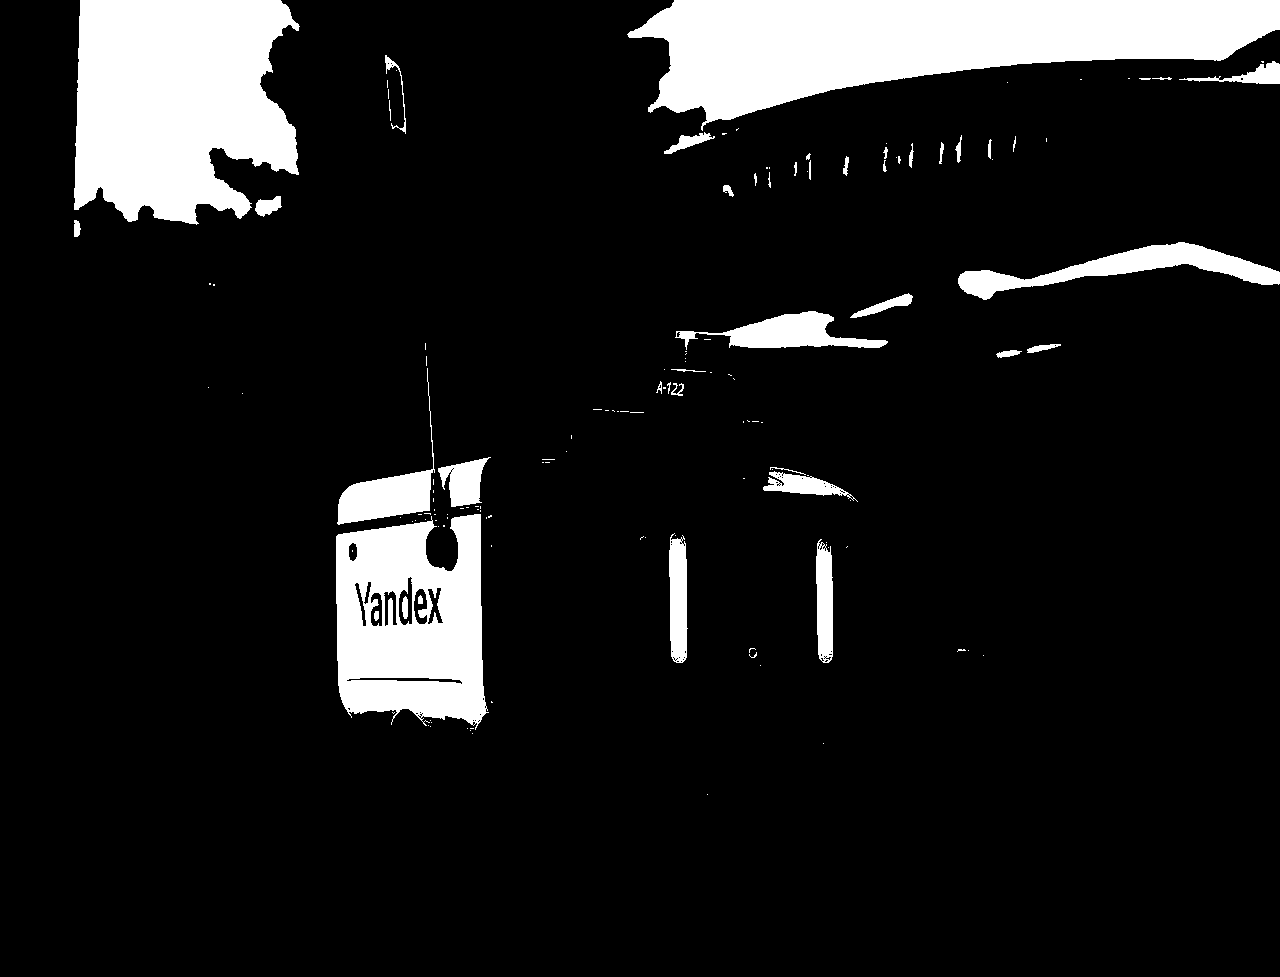
\includegraphics[width=\textwidth]{../outputs/image_double_binarization.png}
    \caption{Бинаризованное изображение по двойному порогу}
    \label{fig:р}
\end{figure}

\begin{lstlisting}[style=cpp_white, caption={Исходный код для бинаризации по двойному порогу, вычисленному статистическим методом Отсу}]
cv::threshold(image, image_new, 0, 255, cv::THRESH_OTSU);

cv::imwrite(path + "/outputs/image_otsu_binarization.png", image_new);
cv::imshow("image", image_new);
cv::waitKey();
\end{lstlisting}

\begin{figure}[ht]
    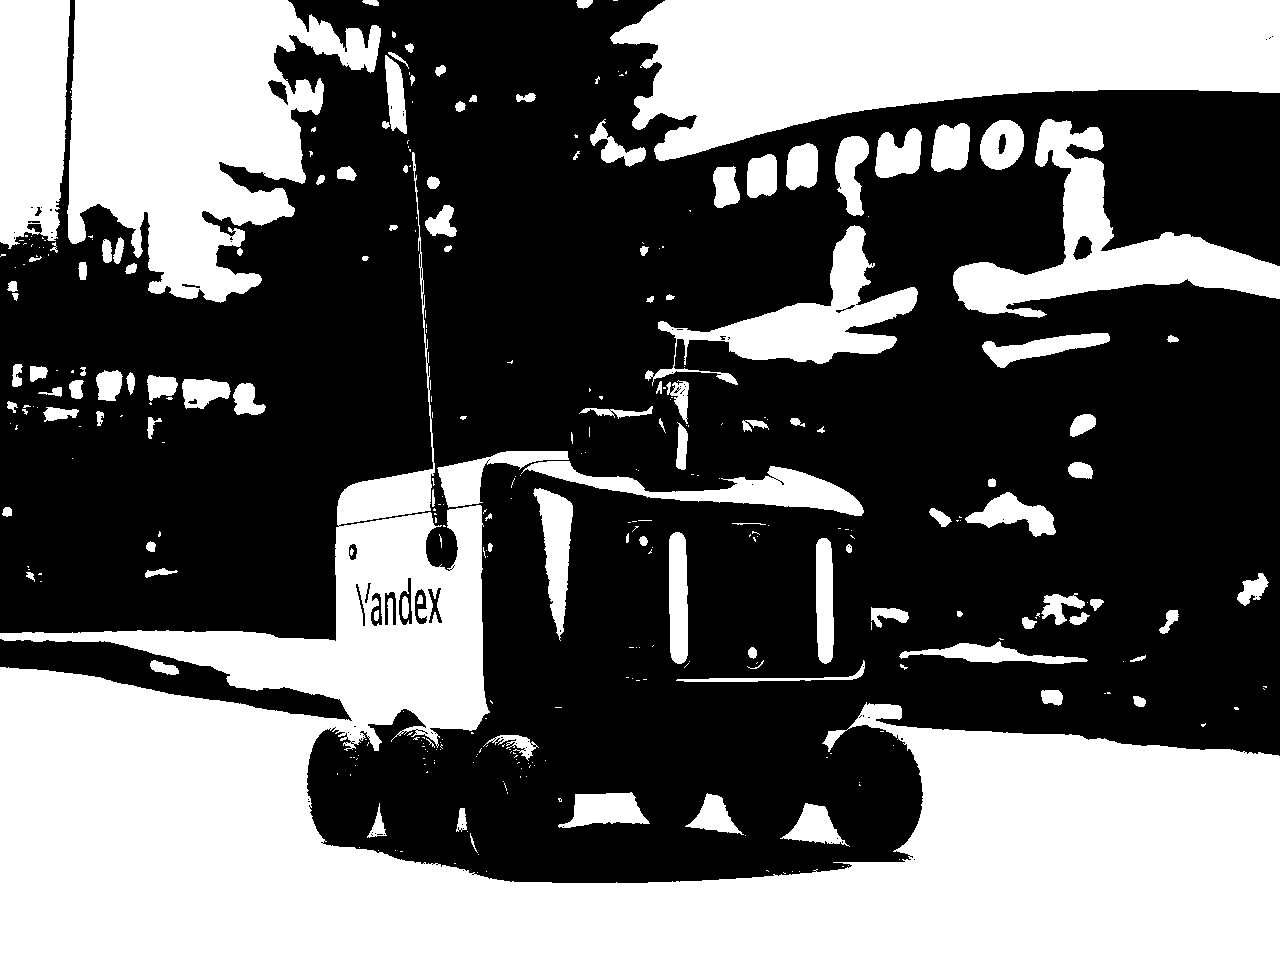
\includegraphics[width=\textwidth]{../outputs/image_otsu_binarization.png}
    \caption{Бинаризованное изображение по двойному порогу, вычисленному по статистическому методу Отсу}
    \label{fig:р}
\end{figure}

\pagebreak

\begin{lstlisting}[style=cpp_white, caption={Исходный код для адаптивной бинаризации}]
cv::threshold(image, image_new, 127, 255, cv::THRESH_TOZERO);
cv::threshold(image_new, image_new, 200, 255, cv::THRESH_BINARY);

cv::imwrite(path + "/outputs/image_double_binarization.png", image_new);
cv::imshow("image", image_new);
cv::waitKey();
\end{lstlisting}

\begin{figure}[ht]
    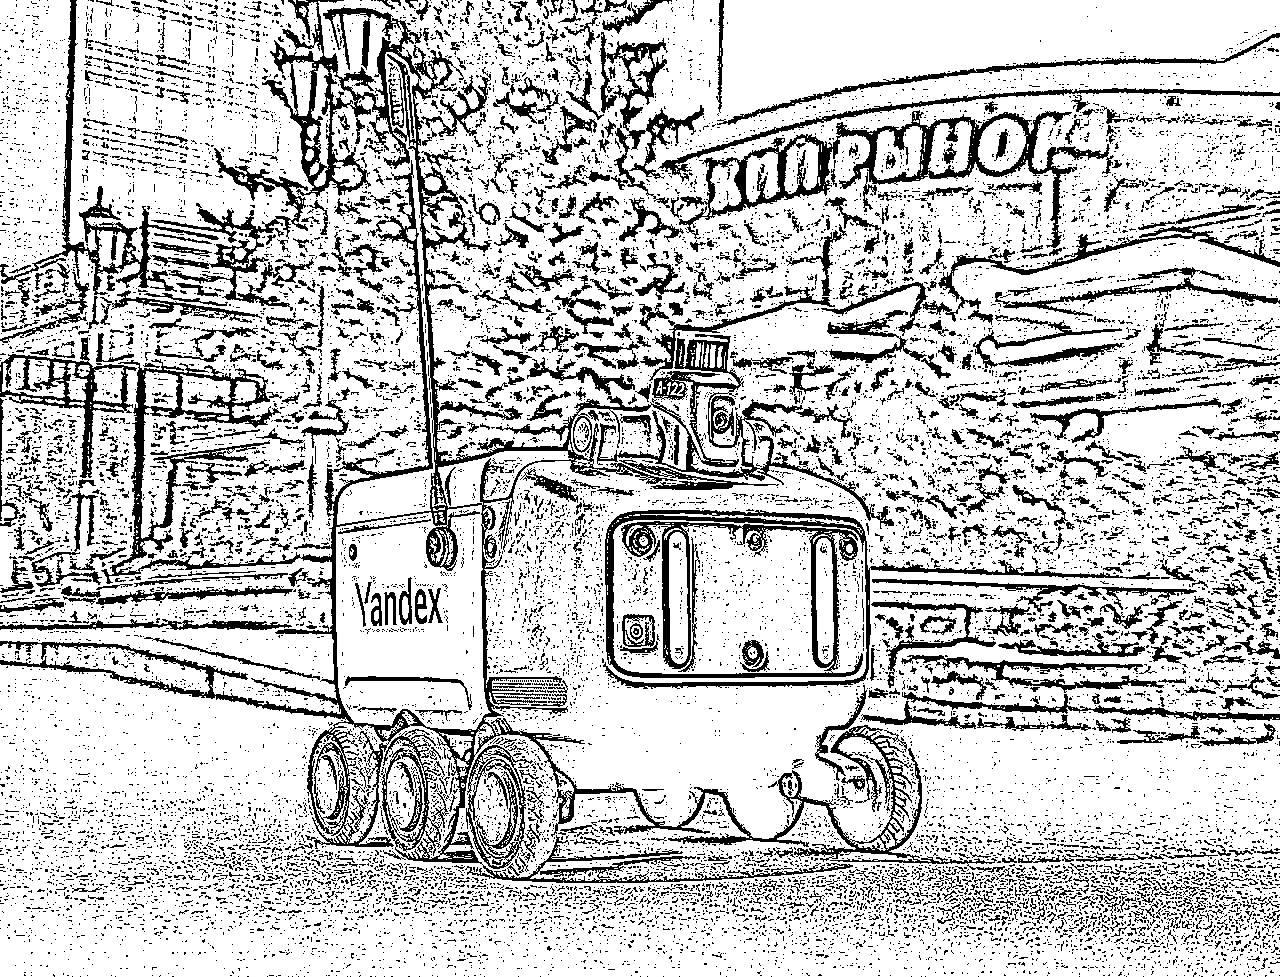
\includegraphics[width=\textwidth]{../outputs/image_adaptive_binarization.png}
    \caption{Бинаризованное изображение адаптивным методом}
    \label{fig:р}
\end{figure}

\pagebreak

\section{Сегментация изображений}

\begin{figure}[ht]
    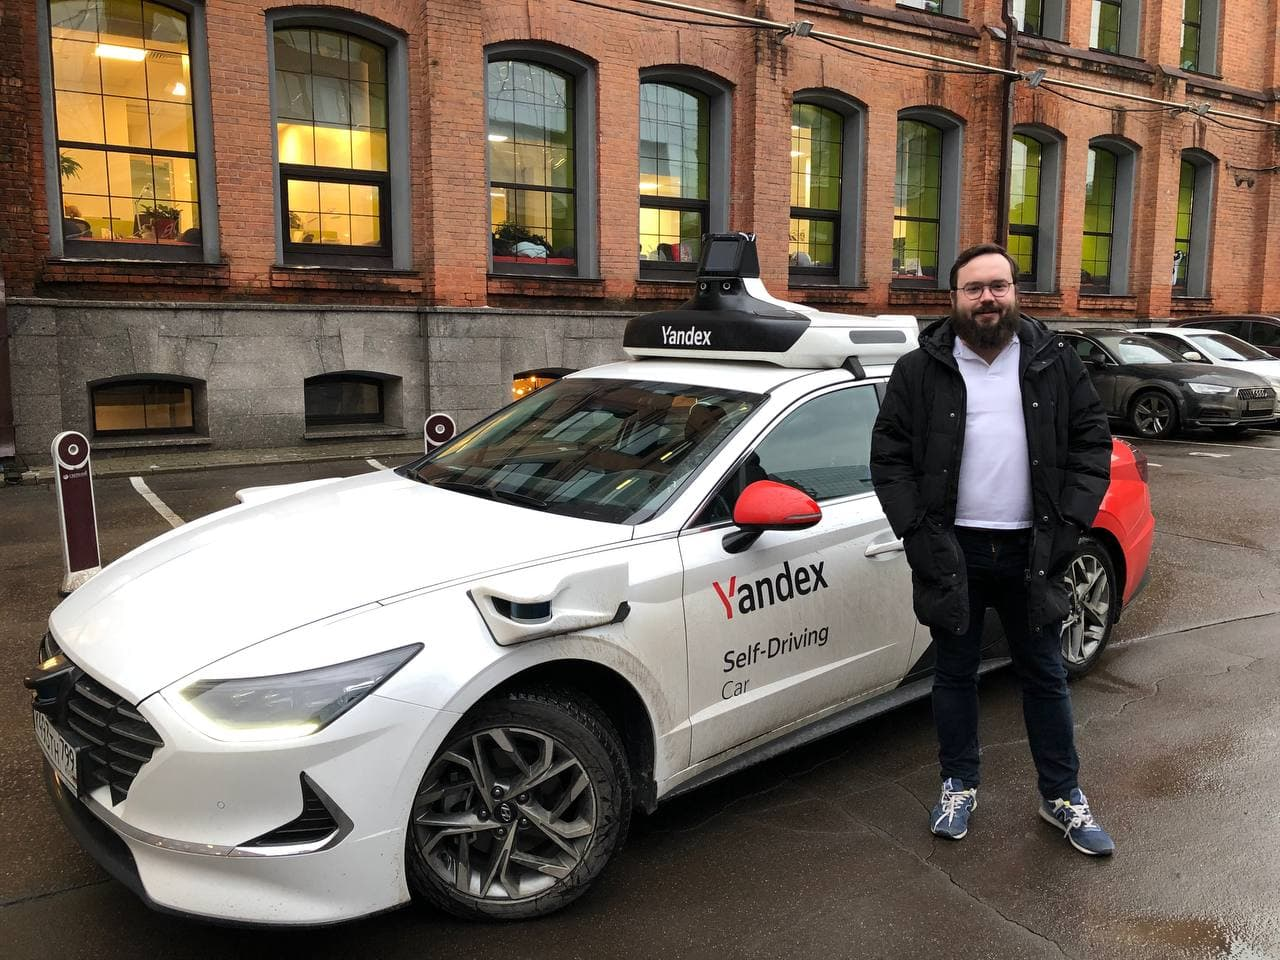
\includegraphics[width=\textwidth]{../source/face.png}
    \caption{Исходное изображение с лицом для сегментации}
    \label{fig:р}
\end{figure}

\subsection{На основе принципа Вебера}

Алгоритм предназначен для сегментации полутоновых изображений. Принцип Вебера подразумевает, что человеческий 
глаз плохо воспринимает разницу уровней серого между $I(n)$ и $I(n)$ + $W(I(n))$, 
где $W(I(n))$ — функция Вебера, $n$ — номер класса, $I$
— кусочно-нелинейная функция градаций серого. Функция Вебе-
ра может быть вычислена по формуле:

\begin{equation}
    W(I) = \begin{cases}
        20 - \frac{12I}{88}, & 0 \leq I \leq 88, \\[1pt]
        0.002(I - 88)^2, & 88 \leq I \leq 138,\\[1pt]
        \frac{7(I - 138)}{117} + 13, & 138 \leq I \leq 255\\[1pt]
    \end{cases} 
\label{eq:complex_func}
\end{equation}

\begin{lstlisting}[style=cpp_white, caption={Исходный код для сегментации по принципу Вебера}]
image = cv::imread(path + "/source/face.png", 0);
image_new = image.clone();

for(int i = 0; i < image_new.rows; ++i){
    for(int j = 0; j < image_new.cols; ++j){
        if(image_new.at<uchar>(i, j) <= 125)
            image_new.at<uchar>(i, j) = 50 - 12 * image_new.at<uchar>(i, j) / 88;   
        
        else if(image_new.at<uchar>(i, j) <= 175)
            image_new.at<uchar>(i, j) = 0.001 * cv::pow(image_new.at<uchar>(i, j) - 88, 2); 
        
        else if(image_new.at<uchar>(i, j) <= 255)
            image_new.at<uchar>(i, j) = 7 * (image_new.at<uchar>(i, j) - 138) / 117; 
    }
}

cv::imwrite(path + "/outputs/image_veber_segmentation.png", image_new);
cv::imshow("image", image_new);
cv::waitKey();
\end{lstlisting}

\begin{figure}[ht]
    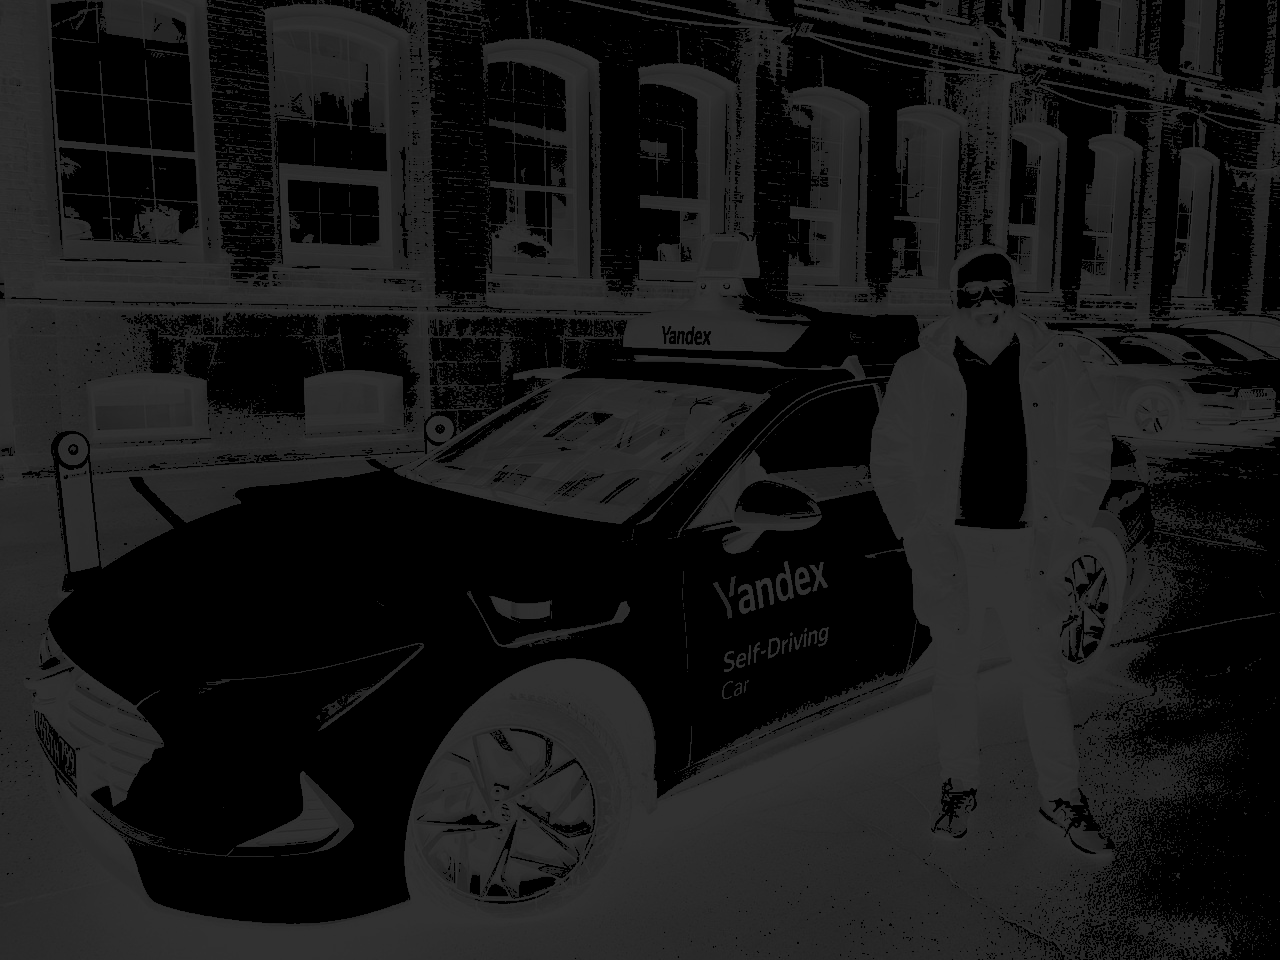
\includegraphics[width=\textwidth]{../outputs/image_veber_segmentation.png}
    \caption{Сегментация изображения по приниципу Вебера}
    \label{fig:р}
\end{figure}

Вероятно, из-за оттенка фона и светлого цвета машины лицо не удалось сегментировать по выбранному алгоритму

\subsection{Сегментация изображения в пространстве CIE Lab по методу k-средних}

Идея метода заключается в определении центров $k$-кластеров и
отнесении к каждому кластеру пикселей, наиболее близко относящихся к этим центрам. Все пиксели рассматриваются как векторы
$x_i$, $i$ = $\overline{1, p}$. Алгоритм сегментации состоит из следующих шагов:

\begin{enumerate}
\item Определение случайным образом $k$ векторов $m_j$, $j$ = $\overline{1, k}$, ко-
торые объявляются начальными центрами кластеров.
\item Обновление значений средних векторов $m_j$ путем вычисления
расстояний от каждого вектора $x_i$ до каждого $m_j$ и их классификации по критерию минимальности расстояния от вектора
до кластера, пересчет средних значений $m_j$ по всем кластерам.
\item Повторение шагов 2 и 3 до тех пора, пока центры кластеров
не перестанут изменяться.
\end{enumerate}

\begin{figure}[ht]
    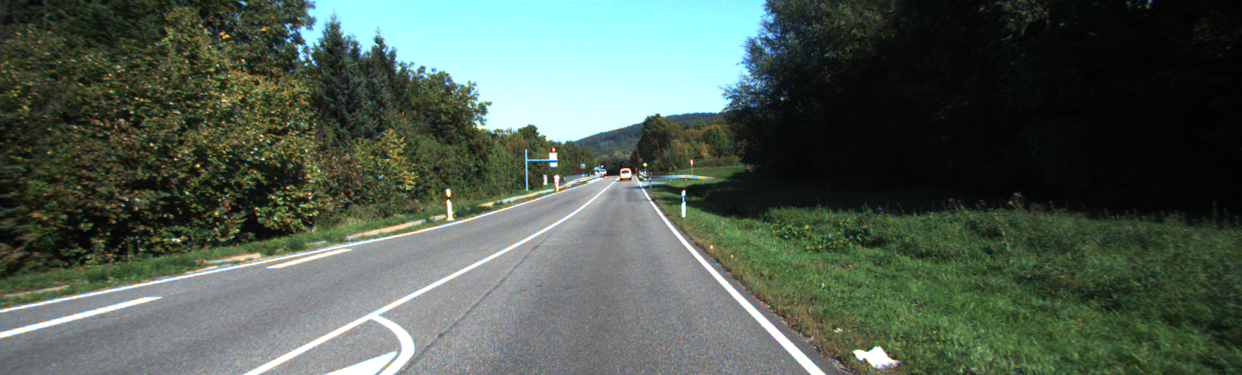
\includegraphics[width=\textwidth]{../source/road.png}
    \caption{Исходное изображение из KITTI Dataset}
    \label{fig:р}
\end{figure}

\begin{lstlisting}[style=cpp_white, caption={Исходный код для сегментации изображения изображения в пространстве CIE Lab по методу k-средних}]
image = cv::imread(path + "/source/road.png", 1);

cv::Mat image_CIE_Lab, ab;
cv::cvtColor(image, image_CIE_Lab, cv::COLOR_BGR2Lab);

std::vector<cv::Mat> image_Lab_canals;
cv::split(image_CIE_Lab, image_Lab_canals);

cv::merge(&(image_Lab_canals[1]), 2, ab);
ab = ab.reshape(0, 1);
ab.convertTo(ab, CV_32F);

int k = 3;
cv::Mat labels;
cv::kmeans(ab, k, labels, cv::TermCriteria(cv::TermCriteria::EPS +
                            cv::TermCriteria::COUNT, 10, 1.0), 10, 
                            cv::KMEANS_RANDOM_CENTERS);

labels = labels.reshape(0, image_Lab_canals[0].rows);

std::vector<cv::Mat> segmentedFrames;
for(int i = 0; i < k; ++i){
    cv::Mat image_tmp = cv::Mat::zeros(image.rows, image.cols, image.type());
    image.copyTo(image_tmp, labels == i);
    segmentedFrames.push_back(image_tmp);
}

cv::imwrite(path + "/outputs/image_CIELab_segmentation.png", segmentedFrames[2]);

cv::threshold(segmentedFrames[2], segmentedFrames[2], 90, 115, cv::THRESH_BINARY);
cv::imwrite(path + "/outputs/image_road_segmentation.png", segmentedFrames[2]);

cv::imshow("image", segmentedFrames[2]);
cv::waitKey();
\end{lstlisting}

\begin{figure}[ht]
    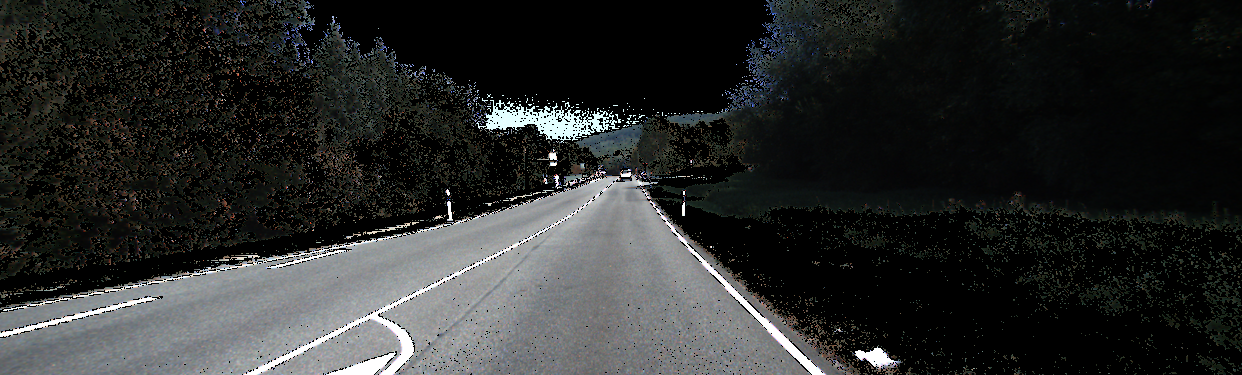
\includegraphics[width=\textwidth]{../outputs/image_CIELab_segmentation.png}
    \caption{Сегментация изображения в пространстве CIE Lab по методу k-средних(составляющая синего оттенка)}
    \label{fig:р}
\end{figure}

\begin{figure}[ht]
    
\includegraphics[width=\textwidth]{../outputs/image_road_segmentation.png}
    \caption{Бинаризация предыдущего изображения для выделения дороги}
    \label{fig:р}
\end{figure}

Если убрать шумы, то будет очень хорошо сегментированная дорога. В случае, когда она пустая, никакие нейронки для сегментации и не нужны.

\pagebreak

\section{Текстурная сегментация}

\begin{figure}[ht]
    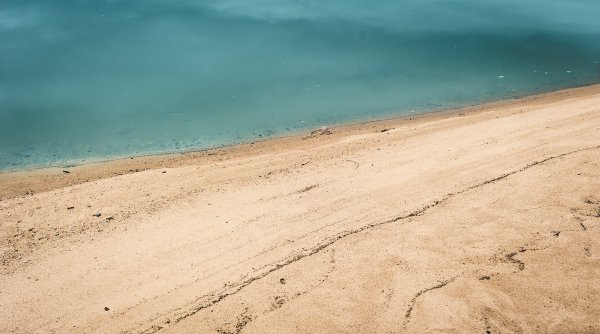
\includegraphics[width=\textwidth]{../source/sea.png}
    \caption{Исходное иображение}
    \label{fig:р}
\end{figure}

\pagebreak

\begin{lstlisting}[style=cpp_white, caption={Текстурная сегментация}]
image = cv::imread(path + "/source/sea.png", 0);

cv::Mat E, Eim;
cv::Mat el = cv::getStructuringElement(cv::MORPH_RECT, cv::Size(9, 9));
entropy(image, E, el);

double Emin, Emax;
cv::minMaxLoc(E, &Emin, &Emax);
Eim = (E - Emin) / (Emax - Emin);
Eim.convertTo(Eim, CV_8U, 255);
cv::Mat BW1;
cv::threshold(Eim, BW1, 0, 255, cv::THRESH_OTSU);

cv::imwrite(path + "/outputs/image_entropy_segmentation.png", BW1);

cv::Mat BWao, closeBWao, Mask1;
bwareaopen(BW1, BWao, 50000);
cv::imwrite(path + "/outputs/image_bwareoopen_segmentation.png", BWao);

cv::Mat nhood = cv::getStructuringElement(cv::MORPH_RECT, cv::Size(9, 9));
cv::morphologyEx(BWao, closeBWao, cv::MORPH_CLOSE, nhood);

imfillholes(closeBWao, Mask1);
cv::imwrite(path + "/outputs/image_imclose_segmentation.png", Mask1);

std::vector<std::vector<cv::Point>> contours;
cv::findContours(Mask1, contours, cv::RETR_TREE, cv::CHAIN_APPROX_NONE);
cv::Mat boundary = cv::Mat::zeros(Mask1.rows, Mask1.cols, CV_8UC1);

cv::drawContours(boundary, contours, -11, 255, 1);
cv::imwrite(path + "/outputs/image_countours_segmentation.png", boundary);

cv::Mat segmentResults = image.clone();
segmentResults.setTo(cv::Scalar(255), boundary != 0);
cv::imwrite(path + "/outputs/image_segmentResults_segmentation.png", segmentResults);

cv::Mat I2 = image.clone();
I2.setTo(0, Mask1 != 0);
\end{lstlisting}

\begin{figure}[H]
    
\includegraphics[width=\textwidth]{../outputs/image_entropy_segmentation.png}
    \caption{Бинаризованное изображение}
    \label{fig:р}
\end{figure}

\begin{figure}[H]
\centering 

\includegraphics[width=\textwidth]{../outputs/image_bwareoopen_segmentation.png}
\caption{Результат выполнения функции bwareaopen()}
\label{fig:р}
\end{figure}

\pagebreak

\begin{figure}[H]
    
\includegraphics[width=\textwidth]{../outputs/image_imclose_segmentation.png}
    \caption{Результат выполнения функции imclose()}
    \label{fig:р}
\end{figure}

\begin{figure}[H]
    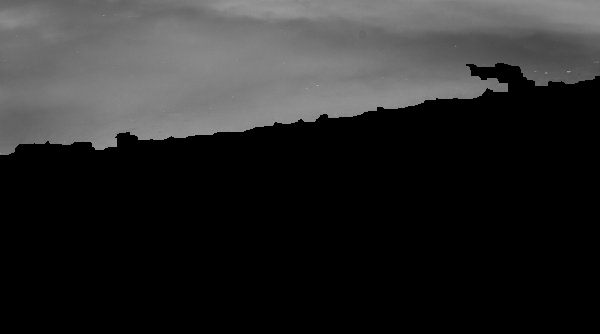
\includegraphics[width=\textwidth]{../outputs/I.png}
    \caption{Результат сегментации воды}
    \label{fig:р}
\end{figure}

\begin{figure}[H]
    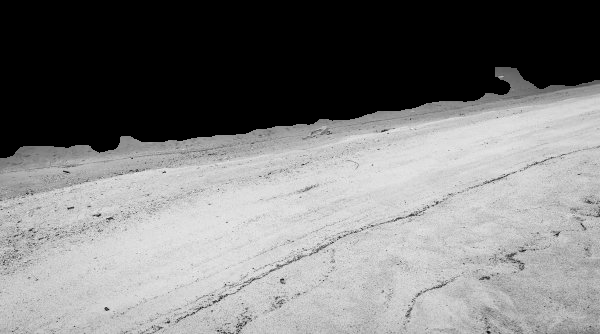
\includegraphics[width=\textwidth]{../outputs/I2.png}
    \caption{Результат сегментации суши}
    \label{fig:р}
\end{figure}

\begin{figure}[hbt!]
    \centering
    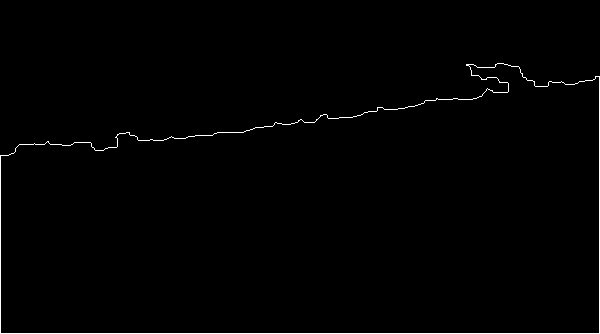
\includegraphics[width=0.6\textwidth]{../outputs/image_countours_segmentation.png}
    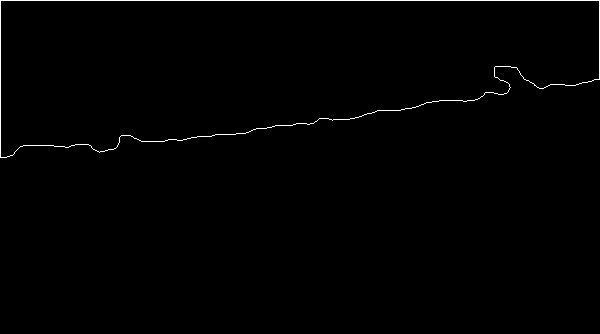
\includegraphics[width=0.6\textwidth]{../outputs/image_countours2_segmentation.png}
    \caption{Выделенные границы текстур относительно воды и суши соответственно}
    \label{fig:stich_images}
\end{figure}

\pagebreak

\subsection{Оценка параметров текстур}

\begin{enumerate}
\item Текстура воды \\
Среднее значение случайной величины = 167.7429504395 \\
Стандартное отклонение = 26.3628025055\\
R - относительная гладкость = 0.0106576710\\
Энтропия гистограммы = 19.4059734344\\

\item Текстура cуши \\
Среднее значение случайной величины = 163.2591247559 \\
Стандартное отклонение = 32.4539321091\\
R - относительная гладкость = 0.0142642801\\
Энтропия гистограммы = 21.3457216344\\
\end{enumerate}


\section{Ответы на вопросы}

\newcounter{question}
\setcounter{question}{0}

\newcommand{\question}[1]{\item[Q\refstepcounter{question}\thequestion.] #1}
\newcommand{\answer}[1]{\item[A\thequestion.] #1}

\begin{itemize}

\question{В каких случаях целесообразно использовать сегментацию попринципу Вебера?}
\answer{Сегментация изображения по принципу Вебера целесообразно использовать в случаях, когда необходимо выделить объекты с малыми различиями в яркости или цвете от фона. Например, в медицинской диагностике для выделения сосудов на рентгеновских изображениях или для распознавания сложных текстур и узоров на изображениях в области компьютерного зрения. Этот метод эффективно работает при анализе изображений с низким контрастом или сложной структурой.}

\question{Какие значения имеют цветовые координаты a и b цветового пространства CIE Lab в полутновом изображении?}
\answer{Значения цветовых координат a и b цветового пространства CIE Lab представляют собой две координаты, определяющие оттенок цвета. Значения этих координат могут изменяться от -128 до 127, где нулевое значение обозначает нейтральный серый цвет. Положительные значения указывают на красные и зеленые оттенки, а отрицательные - на голубые и желтые оттенки.
В полутоновых изображениях, которые имеют только один канал интенсивности, координаты a и b всегда равны нулю, что указывает на отсутствие цвета. Это потому, что полутоновые изображения представляют собой градации серого, а не настоящий цвет.}

\question{Зачем производить сегментацию в цветовом пространстве CIE Lab, а не в исходном RGB?}
\answer{
\begin{enumerate}
Сегментация в цветовом пространстве CIE Lab предпочтительнее, чем в RGB, по следующим причинам:
\item CIE Lab - это универсальное цветовое пространство, которое более близко соответствует восприятию цвета человеческим глазом. Оно разделяет цвет и яркость, что делает его более подходящим для анализа и обработки цвета.
\item В CIE Lab цвета линейно распределены, что упрощает вычисления и обработку цветов. Также это пространство является независимым от устройства, что позволяет достичь более надежных результатов при анализе цвета.
\item CIE Lab позволяет более точно разделять различные цвета и текстуры в изображении, что делает сегментацию более эффективной и точной.

Таким образом, проведение сегментации в цветовом пространстве CIE Lab позволяет добиться более качественных и точных результатов, чем при использовании исходного RGB.
\end{enumerate}
}

\question{Что такое цветовое пространство и цветовой охват?}
\answer{Цветовое пространство – это система координат, которая определяет цвет каждой точки в изображении. Цветовой охват, или цветовая гамма, обозначает диапазон цветов, которые могут быть воспроизведены или отображены в данном цветовом пространстве. Например, RGB (красный, зеленый, синий) – одно из наиболее популярных цветовых пространств, которое включает в себя определенный диапазон цветов, которые могут быть созданы путем комбинирования этих трех основных цветов.}

\end{itemize}

